\documentclass[12pt,a4paper]{article}

% ---------- Kodiranje, jezik, fontovi ----------
\usepackage[T1]{fontenc}
\usepackage[utf8]{inputenc}
\usepackage{babel}
\babelprovide[import,main]{serbian}
\usepackage{mathptmx}
\usepackage[scaled=0.92]{helvet}
\usepackage{microtype}

% ---------- Raspored strane ----------
\usepackage[a4paper,top=2cm,bottom=2cm,left=2.5cm,right=2.5cm]{geometry}
\setlength{\parindent}{1em}
\setlength{\parskip}{0.4em}

% ---------- Paketi ----------
\usepackage{graphicx}
\usepackage{float}
\usepackage{indentfirst}
\usepackage{array}
\usepackage{caption}
\usepackage{titlesec}
\usepackage{hyperref}
\hypersetup{hidelinks}

% ---------- Naslovi poglavlja: "1.   Uvod" ----------
\titleformat{\section}{\sffamily\bfseries\Large}{\thesection.}{1.2em}{}
\titlespacing*{\section}{0pt}{1.4em}{0.5em}

% ---------- Natpisi: "Ilustracija 1." / "Tabela 1." ----------
\captionsetup{labelfont=bf,labelsep=space,font=normalsize}
\captionsetup[figure]{name=Ilustracija,position=below}
\captionsetup[table]{name=Tabela,position=above}
\DeclareCaptionLabelFormat{withdot}{#1 #2.}
\captionsetup{labelformat=withdot}

% ---------- Literatura ----------
\renewcommand{\refname}{References}

\pagestyle{plain}

\begin{document}

% ================= NASLOV =================
\begin{center}
  \rule{\textwidth}{0.4pt}\\[0.8em]
  {\Large\textsc{[Programski prevodioci] Adventure DSL: Domenski specifičan jezik za interaktivnu fikciju sa konzolnim interpreterom i generatorom web igara}}\\[0.6em]
  \rule{\textwidth}{0.4pt}\\[0.8em]

  \begin{tabular}{c@{\hspace{2.5em}}c@{\hspace{2.5em}}c}
    \textbf{Boris Mirković}               & \textbf{Abdurahman Karišik}          & \textbf{Mihajlo Stojanović} \\
    Računarski fakultet                   & Računarski fakultet                  & Računarski fakultet \\
    Univerzitet Union, Beograd, Srbija    & Univerzitet Union, Beograd, Srbija   & Univerzitet Union, Beograd, Srbija \\
    (studentski mejl)                     & (studentski mejl)                    & m\_stojanovic@raf.rs \\
  \end{tabular}\\[0.3em]
\end{center}

% ================= APSTRAKT =================
\begin{center}
  {\sffamily\bfseries\large Apstrakt}
\end{center}
\begin{list}{}{\leftmargin=2.2cm \rightmargin=2.2cm}
\item[]\small
U radu je predstavljen Adventure DSL, deklarativni domenski specifičan jezik namenjen kreiranju tekstualnih avantura i interaktivne fikcije. Razvijen je kompletan prevodilački sistem koji obuhvata leksičku analizu, rekurzivni silazni parser sa apstraktnim sintaksnim stablom i semantičku analizu sa statičkom proverom tipova. Generička faza podržava dva pristupa: direktno interpretiranje u konzolnom okruženju i generisanje samostalnih web aplikacija u formatu HTML5 i JavaScript. Rešenje je uspešno evaluirano na deset reprezentativnih scenarija i pokriveno automatizovanim testovima, čime se dokazuje jednostavnost pisanja interaktivnih priča uz očuvanje potpune tipovske i semantičke sigurnosti.

\medskip
\noindent\textbf{Ključne reči}: domenski specifičan jezik, interaktivna fikcija, rekurzivni silazni parser, semantička analiza, generator koda, interpreter
\end{list}

% ================= 1. UVOD =================
\section{Uvod}
Interaktivna narativna fikcija i tekstualne avanture predstavljaju jedan od najstarijih i najuticajnijih žanrova računarskih igara, u kojima se igrač kroz priču kreće donošenjem tekstualnih odluka i upravljanjem stanjem virtuelnog sveta~\cite{montfort2005twisty}. Iako savremena industrija video-igara dominira vizuelnim i trodimenzionalnim okruženjima, tekstualne avanture doživljavaju renesansu u domenima digitalne književnosti, interaktivnog učenja i brzog prototipovanja narativa~\cite{short2014interactive}. Razvoj ovakvih sistema u jezicima opšte namene, poput C++ ili Pythona, često zahteva pisanje obimnog koda za upravljanje grafom lokacija, inventarom i logičkim uslovima, što stvara visoku barijeru za autore priča koji ne poseduju formalno programersko obrazovanje~\cite{aho2006compilers}. Domenski specifični jezici (DSL) nude elegantan odgovor na ovaj izazov, jer omogućavaju formulisanje koncepata direktno kroz rečnik problema, apstrahujući mehanizme alokacije memorije i složenih upravljačkih struktura~\cite{fowler2010domain}.

U oblasti sistema za razvoj interaktivne fikcije postoji nekoliko prepoznatljivih alata i platformi. Istorijski najznačajniji pristup potiče od Infocom Z-Machine virtuelne mašine, koja je omogućila prenosivost tekstualnih igara na različite hardverske arhitekture sedamdesetih i osamdesetih godina prošlog veka~\cite{nelson2001inform}. Tokom dvehiljaditih godina razvijen je Inform 7, revolucionarni sistem koji koristi sintaksu zasnovanu na prirodnom engleskom jeziku~\cite{nelson2006natural}. Pored njega, široku popularnost stekao je Twine, alat usmeren na hipertekstualne nelinearne narative u veb formatu~\cite{klimas2014twine}, kao i Ink, deklarativni skripting jezik koji je studio Inkle razvio za potrebe integracije u savremene grafičke pogone poput Unity-ja~\cite{inkle2016ink}. Istraživanja u oblasti prevodilaca za narativne jezike pokazuju stalnu potrebu za balansiranjem između izražajnosti sintakse i formalne verifikacije logičkih stanja pre samog pokretanja igre~\cite{wardrip2006expressive}.

Ipak, postojeći alati često pate od izražene asimetrije: ili zahtevaju učenje složenih sintaksnih koncepata i glomaznih alata za prevođenje, ili se oslanjaju na vizuelne blokove koji postaju nepregledni sa rastom broja grana u priči. Značaj našeg rada ogleda se u konstrukciji kompaktnog, formalno verifikovanog domenskog jezika Adventure DSL koji autorima pruža minimalističku i čitljivu sintaksu na maternjem jeziku, uz potpuno statičku semantičku proveru integriteta celokupnog grafa priče pre njenog pokretanja. Dodatna vrednost ovog rešenja leži u podršci za dvostruko generičko izvođenje — omogućeno je i trenutno terminalno izvršavanje kroz ugrađeni interpreter, kao i automatska sinteza samostalne veb igre zasnovane na HTML5 i JavaScript tehnologijama koja ne zahteva instalaciju ikakvog dodatnog softvera na strani krajnjeg korisnika.

% ================= 2. SRODNI RADOVI =================
\section{Srodni radovi}
Detaljnija analiza postojećih rešenja otkriva jasne funkcionalne praznine koje motivišu razvoj našeg prevodioca. Sistem Inform 7 uveo je ambiciozan koncept programiranja na prirodnom engleskom jeziku, ali se u praksi pokazalo da takva sintaksa stvara privid fleksibilnosti, dok u stvarnosti nameće stroga i često neintuitivna gramatička ograničenja koja dovode do teških leksičkih i sintaksnih nejasnoća pri kompajliranju~\cite{nelson2006natural, montfort2005twisty}. Sa druge strane, alati poput Twine-a~\cite{klimas2014twine} pružaju odličnu veb distribuciju, ali pate od potpunog nedostatka statičke provere tipova i integriteta promenljivih; greške u nazivima lokacija ili promenljivih stanja u Twine-u manifestuju se tek u toku samog igranja u pretraživaču, što otežava debagovanje obimnih priča. Jezik Ink~\cite{inkle2016ink} pruža moćne mehanizme za grananje dijaloga, ali je primarno zamišljen kao podsistem koji se mora ugraditi u veći programski okvir (poput C\# biblioteke) i ne poseduje sopstvenu samostalnu infrastrukturu za direktno generisanje gotovih igara. U ovom radu predstavljamo Adventure DSL kao rešenje koje objedinjuje najbolje osobine navedenih pristupa: formalnu EBNF gramatiku koja sprečava sintaksne dvosmislenosti, rigoroznu semantičku proveru simbola i tipova pre izvršavanja, te dvostruku generičku fazu koja istovremeno nudi terminalsku interakciju za autora i veb distribuciju za publiku.

% ================= 3. METODOLOGIJA =================
\section{Metodologija}
Razvoj prevodioca za Adventure DSL organizovan je prema klasičnim principima teorije programskih prevodilaca, kroz tri analitičke faze (leksička, sintaksna i semantička analiza) i dve komplementarne generičke faze (direktno interpretiranje i generisanje koda u ciljnom jeziku). Celokupan sistem implementiran je u programskom jeziku Python korišćenjem isključivo standardne biblioteke, bez oslanjanja na spoljne generatore parsera poput ANTLR-a ili Flex/Bison alata, čime je postignuta maksimalna kontrola nad prijavljivanjem grešaka i prenosivošću.

\begin{figure}[H]
  \centering
  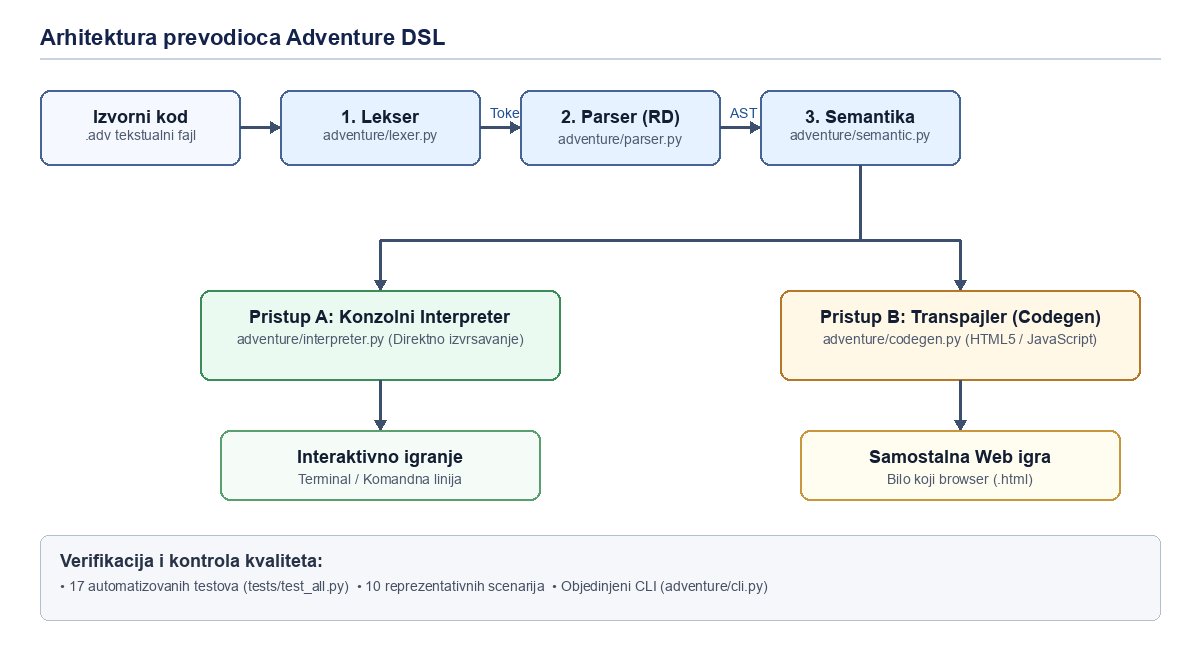
\includegraphics[width=0.92\textwidth]{arhitektura.png}
  \caption{Arhitektura prevodioca Adventure DSL i tok faza obrade.}
  \label{fig:arhitektura}
\end{figure}

Kao što je prikazano na Ilustraciji~\ref{fig:arhitektura}, proces obrade započinje prijemom izvornog koda sa ekstenzijom \texttt{.adv}. Prva faza je leksička analiza, poverena klasi \texttt{Lexer}. Lekser sekvencijalno analizira ulazni niz karaktera i pretvara ga u tok tokena, pri čemu beleži tačne pozicije svakog tokena kroz broj linije i kolone radi kasnijeg preciznog lokalizovanja grešaka. U ovoj fazi prepoznaju se rezervisane ključne reči jezika (\texttt{STORY}, \texttt{START\_LOCATION}, \texttt{ITEMS}, \texttt{LOCATION}, \texttt{OPTION}, \texttt{SET}, \texttt{IF}, itd.), identifikatori sa punom podrškom za lokalizovane latinične karaktere (\texttt{č}, \texttt{ć}, \texttt{ž}, \texttt{š}, \texttt{đ}), celobrojni literali, stringovi sa eskejp sekvencama, kao i jednoznačni i dvoetapni operatori (\texttt{==}, \texttt{!=}, \texttt{<=}, \texttt{>=}). Beline i jednolinijski komentari koji počinju simbolom tarabe se automatski uklanjaju.

Druga faza je sintaksna analiza, realizovana kroz rekurzivni silazni parser (\texttt{Parser}). Parser prihvata niz tokena i transformiše ga u strogo tipizirano apstraktno sintaksno stablo (AST). Gramatika jezika definisana je u proširenoj Bakus-Nurovoj formi (EBNF) kao LL(1) gramatika bez leve rekurzije. Izrazi su stratifikovani u osam nivoa prioriteta: od logičkog disjunkta (\texttt{OR}) na najnižem nivou, preko konjunkcije (\texttt{AND}), relacija jednakosti i poređenja, do aritmetičkih operacija sabiranja, množenja, unarnih operatora (\texttt{NOT}, unarni minus) i primarnih izraza (\texttt{HAS}, literali, promenljive i zagrade). Svaki čvor u stablu nasleđuje baznu klasu \texttt{ASTNode} i čuva podatke o liniji i koloni gde je pravilo prepoznato.

Treća analitička faza jeste semantička analiza (\texttt{SemanticAnalyzer}). Njen zadatak je statička validacija značenja programa pre pokretanja. Analizator formira tri ključne strukture simbola: mapu lokacija (\texttt{locations\_map}), skup deklarisanih predmeta (\texttt{items\_set}) i tabelu simbola stanja (\texttt{symbol\_table}). Tokom obilaska stabla, analizator vrši izvođenje tipova (\emph{Type Inference}) na osnovu početnih vrednosti promenljivih u bloku \texttt{STATE} i proverava: postojanje početne lokacije \texttt{START\_LOCATION}, jedinstvenost lokacija i opcija, ispravnost skokova \texttt{GOTO}, deklarisanost predmeta u naredbama \texttt{ADD\_ITEM}, \texttt{REMOVE\_ITEM} i izrazima \texttt{HAS}, kao i slaganje tipova u naredbama dodele \texttt{SET} i uslovima grananja \texttt{IF} i \texttt{WHILE} (koji moraju biti logičkog tipa).

Generička faza nudi dva nezavisna modaliteta izvođenja. Prvi pristup je konzolni interpreter (\texttt{Interpreter}), koji obilazi verifikovano stablo i neposredno simulira virtuelni svet kroz interakciju sa korisnikom u komandnoj liniji, vodeći evidenciju o promenljivim stanja, inventaru i dinamičkom otključavanju opcija uz prikaz saveta (\texttt{HINT}). Drugi pristup predstavlja generator koda (\texttt{HTMLCodeGenerator}) koji prevodi celokupno AST stablo u samostalnu veb aplikaciju sa HTML5 strukturom, CSS stilizacijom i optimizovanim JavaScript pogonom koji u pretraživaču emulira identičnu semantiku izvršavanja.

% ================= 4. PRELIMINARNI REZULTATI =================
\section{Preliminarni rezultati}
Evaluacija razvijenog prevodilačkog sistema sprovedena je na korpusu od deset raznovrsnih scenarija interaktivnih priča (\texttt{01\_tvrdjava.adv} do \texttt{10\_svetionik.adv}), koji pokrivaju različite aspekte jezika: ciklične lavirinte, zagonetke sa inventarom, simulaciju protoka vremena kroz petlje i grananja zasnovana na vrednostima unutrašnjeg stanja. Dodatno, formiran je automatizovani test paket od 17 jediničnih i integracionih testova (\texttt{tests/test\_all.py}) koji testira robusnost leksera, parsera, semantičkog analizatora i oba generička podsistema.

\begin{table}[H]
  \centering
  \caption{Komparativna evaluacija dva pristupa izvođenja jezika Adventure DSL.}
  \label{tab:evaluacija}
  \renewcommand{\arraystretch}{1.3}
  \begin{tabular}{|p{0.48\textwidth}|c|c|}
    \hline
    \textbf{Kriterijum evaluacije} & \textbf{Konzolni interpreter} & \textbf{HTML/JS Transpajler} \\ \hline
    Vreme inicijalnog pokretanja & $<$ 0.05 s & Trenutno (u browseru) \\ \hline
    Zavisnost od radnog okruženja & Zahteva Python 3.10+ & Bez zavisnosti (bilo koji browser) \\ \hline
    Prenosivost na mobilne uređaje & Ograničena (zahteva terminal) & Potpuna (odzivni veb interfejs) \\ \hline
    Korisnički doživljaj (UI/UX) & Tekstualan (ASCII/ANSI) & Grafički (dugmad, bedževi, animacije) \\ \hline
    Lokalizacija i debagovanje grešaka & Detaljna (linija, kolona, stog) & Statička (pre samog eksporta) \\ \hline
    Veličina generisanog artefakta & Nema dodatnog fajla & 12 -- 14 KB (jedan HTML fajl) \\ \hline
  \end{tabular}
\end{table}

Kao što je prikazano u Tabeli~\ref{tab:evaluacija}, uporedna analiza dva pristupa otkriva njihove komplementarne prednosti. Konzolni interpreter omogućava trenutno pokretanje koda tokom procesa pisanja priče i pruža vrhunsko okruženje za debagovanje, jer direktno u terminalu ispisuje detaljne semantičke i sintaksne greške sa tačnim brojem linije i kolone. Sa druge strane, HTML/JavaScript generator koda postiže superiornu distribuciju: izlazni artefakt je kompaktan pojedinačni HTML fajl veličine svega 12 do 14 kilobajta, koji sadrži kompletnu logiku igre i moderan taman korisnički interfejs. Ovaj veb artefakt je potpuno autonoman, ne zahteva veb server niti baze podataka, i besprekorno funkcioniše na svim savremenim stonim i mobilnim internet pretraživačima. Svi testirani scenariji su uspešno prevedeni i verifikovani u oba režima izvođenja.

% ================= 5. DISKUSIJA =================
\section{Diskusija}
Iako je Adventure DSL postigao planirane ciljeve u pogledu jednostavnosti sintakse i statičke sigurnosti, uočena su određena funkcionalna ograničenja u trenutnoj arhitekturi. Sistem trenutno podržava isključivo celobrojnu aritmetiku, dok realni brojevi sa pokretnim zarezom nisu podržani jer nisu bili neophodni za analizirane narativne obrasce; u budućim verzijama podrška za decimalne vrednosti može se uvesti proširenjem leksičkog automata i tabele simbola. Takođe, jezik trenutno ne podržava korisnički definisane potprograme i funkcije, već se modularnost postiže strukturiranjem lokacija i skokova, što pri veoma složenim nelinearnim zapletima može dovesti do redundancije u telima opcija. Ipak, postignuti rezultati u potpunosti potvrđuju navode iz odeljka o srodnim radovima: eliminisane su semantičke dvosmislenosti svojstvene Informu 7, obezbeđena je rigorozna statička kontrola tipova koja nedostaje sistemu Twine, i kreiran je autonoman generator koda koji ne zavisi od eksternih grafičkih mehanizama poput Inka.

% ================= 6. ZAKLJUČAK =================
\section{Zaključak}
U ovom radu uspešno je dizajniran i implementiran domenski specifičan jezik Adventure DSL, zajedno sa kompletnim prevodilačkim sistemom koji obuhvata analitičke i generičke faze. Dokazano je da je primenom formalne EBNF gramatike, rekurzivnog silaznog parsiranja i statičke provere tipova moguće autorima pružiti izuzetno pristupačan i intuitivan alat za interaktivnu fikciju, uz istovremenu garanciju semantičke korektnosti programa. Kao pravci budućeg razvoja izdvajaju se implementacija vizuelnog editora grafa lokacija sa dvosmernom sinhronizacijom izvornog koda, proširenje tipskog sistema strukturiranim podacima i dodavanje modula za automatsko generisanje grafičke mape sveta na osnovu definisanih relacija prelaza.

% ================= 7. ZAHVALNOSTI =================
\section{Zahvalnosti}
Autori izražavaju zahvalnost saradniku u nastavi Mihajlu Stojanoviću na stručnim savetima, smernicama tokom semestra i definisanju formalnog okvira za izradu malog naučnog rada. Takođe, u skladu sa tehničkom specifikacijom predmeta, navodi se da su alati veštačke inteligencije (konkretno Gemini) korišćeni kao pomoćni instrumenti pri debagovanju programskog koda leksera i parsera, proveri gramatičke korektnosti teksta i generisanju vektorskog dijagrama arhitekture, dok su celokupna koncepcija jezika, logika prevodioca i sinteza zapažanja delo autora.

% ================= 8. REFERENCES =================
\section{References}
\begingroup
\renewcommand{\section}[2]{}
\begin{thebibliography}{9}
  \bibitem{montfort2005twisty}
  N.~Montfort, \emph{Twisty Little Passages: An Approach to Interactive Fiction}. Cambridge, MA, USA: MIT Press, 2005.

  \bibitem{short2014interactive}
  E.~Short, ``Interactive Fiction: The Future of Narrative Games,'' in \emph{Proceedings of the IEEE International Games Innovation Conference (IGIC)}, Rochester, NY, USA, 2014, pp.~1--6.

  \bibitem{aho2006compilers}
  A.~V.~Aho, M.~S.~Lam, R.~Sethi, and J.~D.~Ullman, \emph{Compilers: Principles, Techniques, and Tools}, 2nd~ed. Boston, MA, USA: Addison-Wesley, 2006.

  \bibitem{fowler2010domain}
  M.~Fowler, \emph{Domain-Specific Languages}. Boston, MA, USA: Addison-Wesley Professional, 2010.

  \bibitem{nelson2001inform}
  G.~Nelson, \emph{The Inform Designer's Manual}, 4th~ed. St. Charles, IL, USA: The Interactive Fiction Library, 2001.

  \bibitem{nelson2006natural}
  G.~Nelson, ``Natural Language, Semantic Analysis, and Interactive Fiction,'' \emph{Literary and Linguistic Computing}, vol.~21, no.~1, pp.~33--48, 2006.

  \bibitem{klimas2014twine}
  C.~Klimas, ``Twine: An Open-Source Tool for Telling Interactive, Nonlinear Stories,'' \url{https://twinery.org/}, 2014, pristupljeno: 2026.

  \bibitem{inkle2016ink}
  J.~Ingold and M.~Humphreys, ``Ink: An Open-Source Scripting Language for Writing Interactive Narrative,'' Inkle Studios, \url{https://github.com/inkle/ink}, 2016, pristupljeno: 2026.

  \bibitem{wardrip2006expressive}
  N.~Wardrip-Fruin, ``Expressive Processing: On Process-Intensive Literature and Digital Games,'' Ph.D. dissertation, Brown University, Providence, RI, USA, 2006.
\end{thebibliography}
\endgroup

\end{document}
